% !TEX TS-program = xelatex
% !TEX encoding = UTF-8 Unicode
% !Mode:: "TeX:UTF-8"
\documentclass{resume}
\usepackage{graphicx}
\usepackage{tabu}
\usepackage{multirow}
\usepackage{progressbar}
\usepackage{zh_CN-Adobefonts_external}
\usepackage{linespacing_fix}
\usepackage{cite}

\begin{document}
\pagenumbering{gobble}

% \name{周伟林}
% \basicInfo{
%   \homepage[zhouweilin.cn]{https://zhouweilin.cn/}\
%   \github[github.com/Si3ver]{https://github.com/Si3ver} 
% }
% \basicInfo{
%   \email{izhouwl@163.com}\ 
%   \phone{176-0053-5912}
% }

\Large{
  \begin{tabu}{ c  l  r }
    \multirow{5}{1.5in}{
       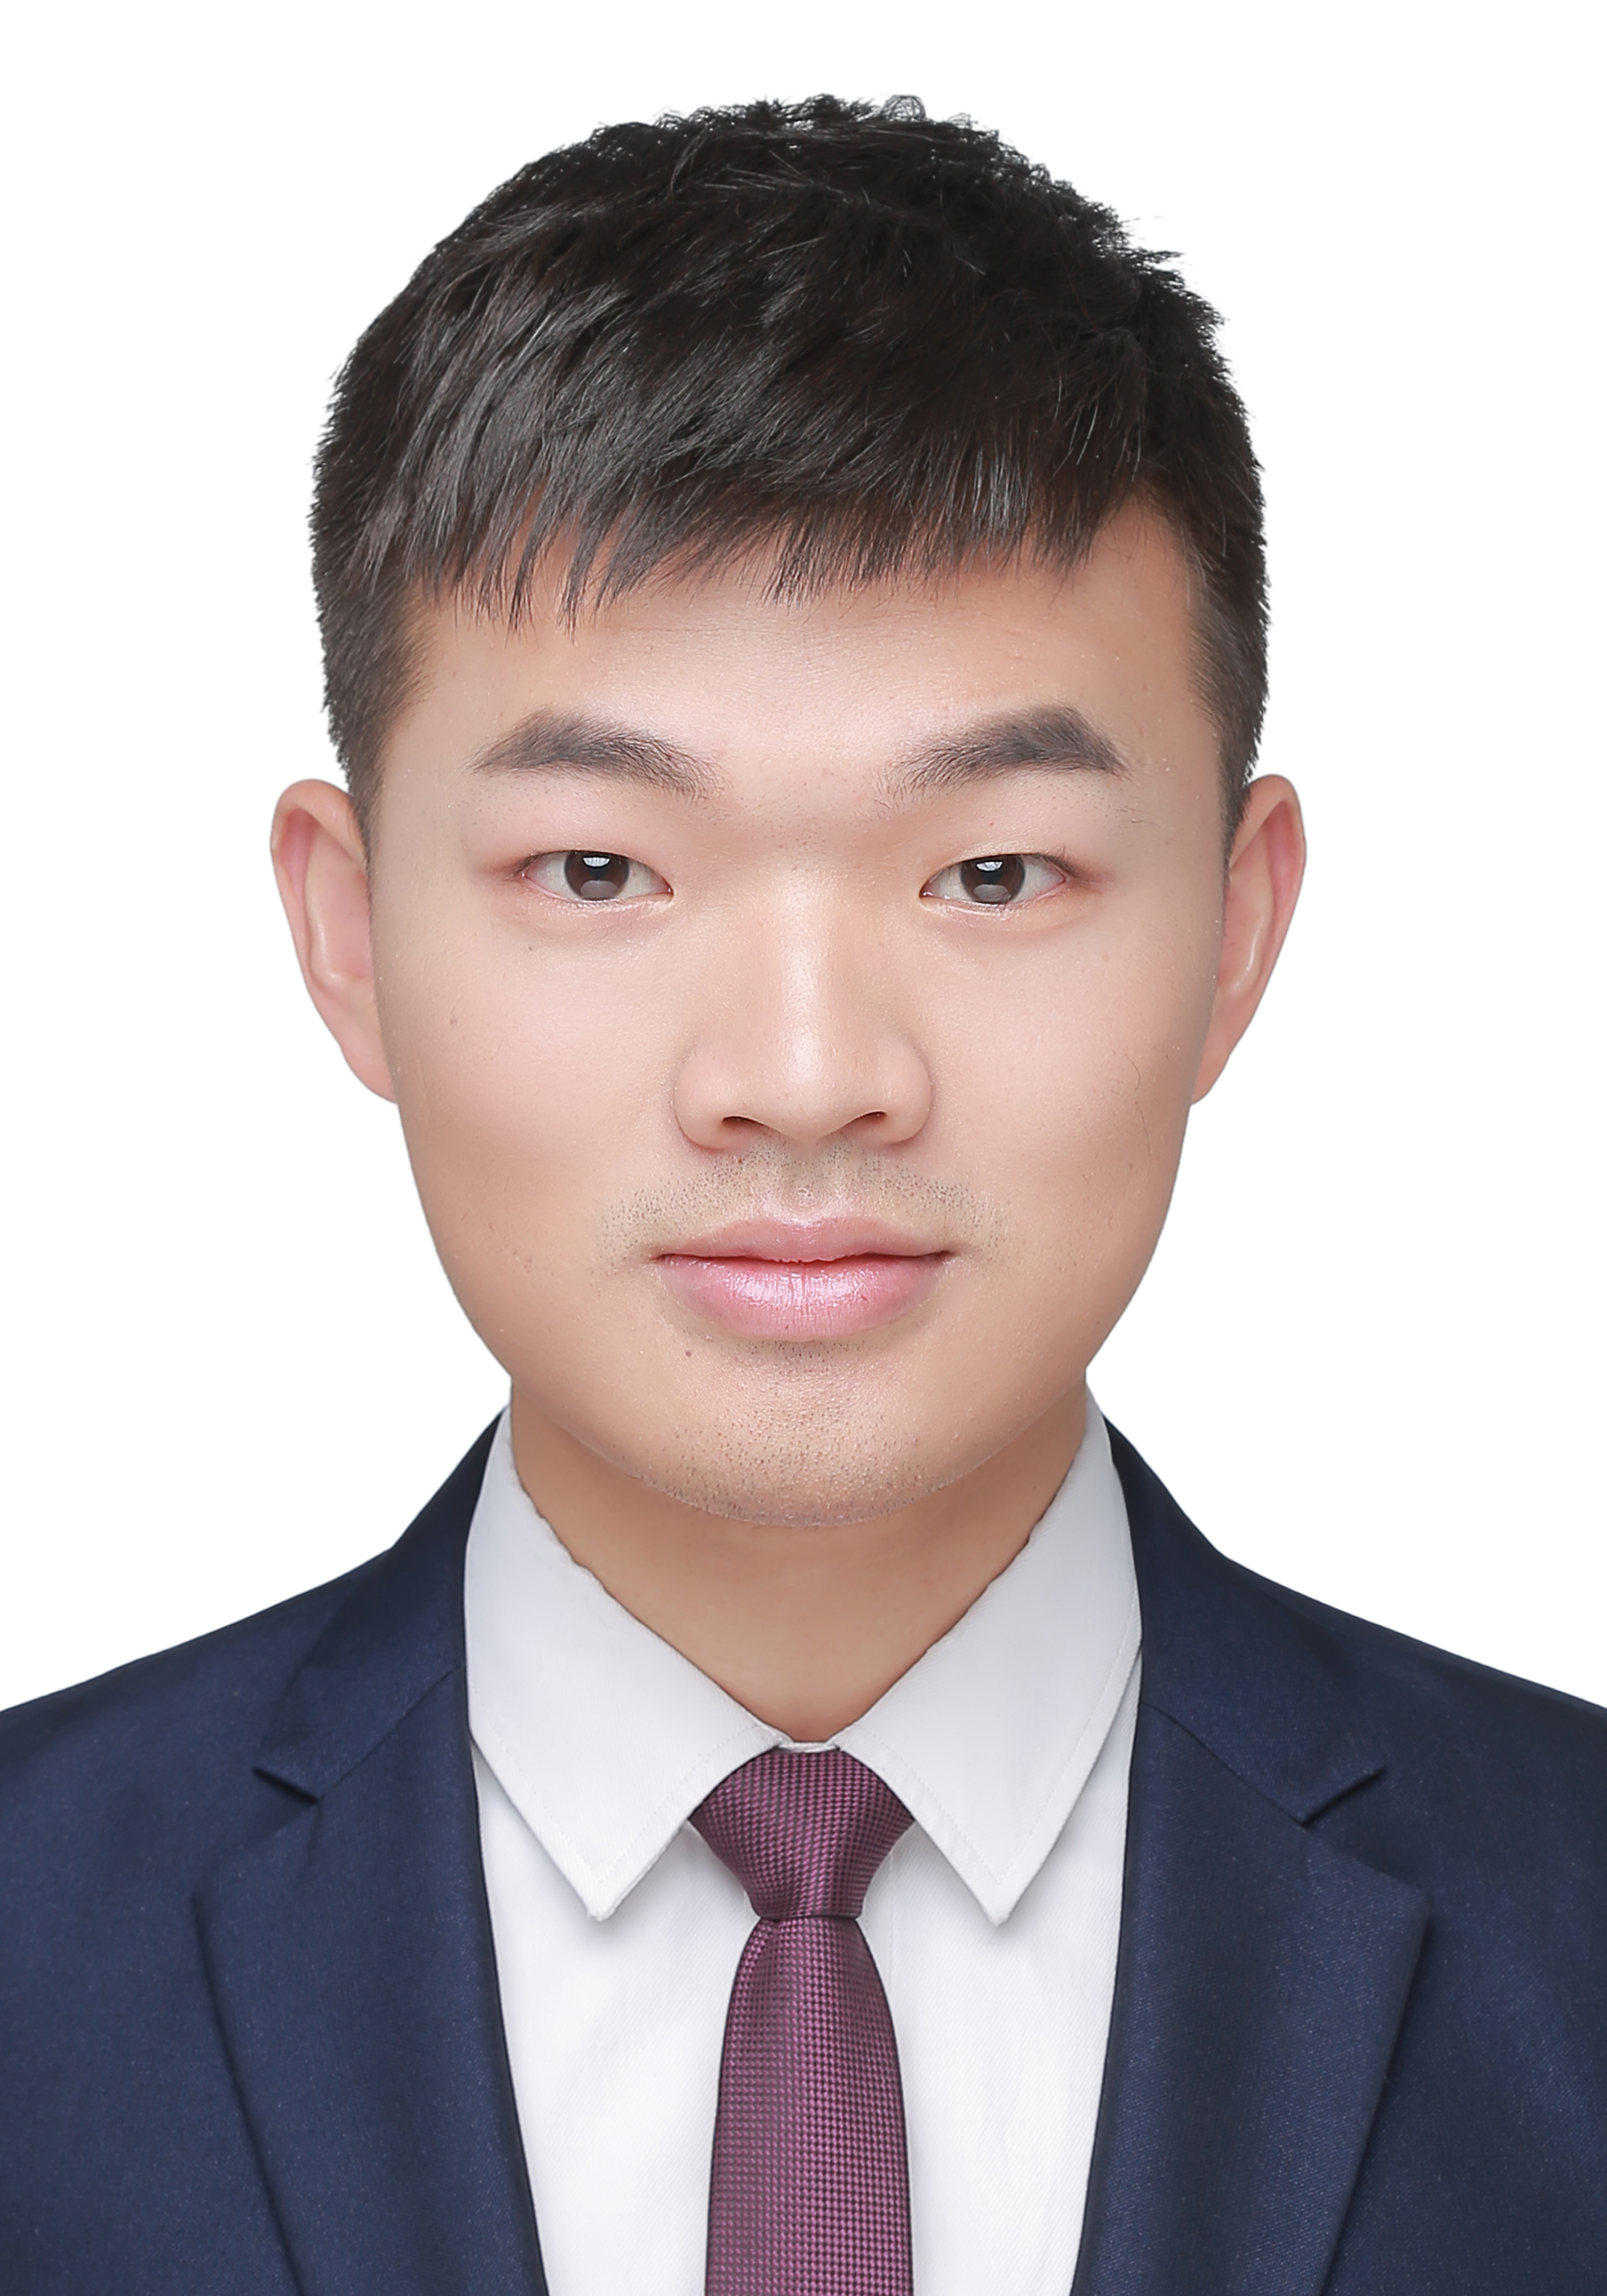
\includegraphics[width=0.88in]{avatar}
    }
    & \scshape{周伟林(前端岗)}
        & {JavaScript~}\progressbar{0.85} \\
    & \email{izhouwl@163.com \quad\quad\quad} 
        & {FEED~}\progressbar{0.7} \\
    & \phone{(+86)17801071698} 
        & {React~}\progressbar{0.7} \\
    & \homepage[www.zhouweilin.cn]{https://zhouweilin.cn} 
        & {python~}\progressbar{0.65} \\
    & \github[github.com/Si3ver]{https://github.com/Si3ver} 
        & {network~}\progressbar{0.9}
  \end{tabu}
}

% 专业技能
\section{\faCogs\ 其他技能}
% increase linespacing [parsep=0.5ex]
\begin{itemize}[parsep=0.5ex]
  \item 熟悉原生JS、ES6、Bootstrap、ECharts、AntD、jQuery、Matplotlib
  \item 会使用Redux、Canvas、Webpack、LaTex
  \item 英语能力,无障碍阅读英文文档,CET-6
%   \item 熟悉HTML5、CSS3、JavaScript、Bootstrap、jQuery,eCharts,了解Canvas
%   \item 熟悉Git、Emmet、ESlint、MS Office、Markdown、LaTex等工具的使用
%   \item 熟悉python 3,了解node.js
%   \item 无障碍阅读英文文档,CET-6
\end{itemize}

% 教育背景
\section{\faGraduationCap\  教育背景}
\datedsubsection{\textbf{北京邮电大学(211)\quad}{ 网研院\quad\quad }{ 计算机科学技术\quad }{ 硕士 }}{2016年09月 -- 2019年06月}
\datedsubsection{\textbf{北京工业大学(211)\quad}{ 计算机院\quad }{ 信息安全\quad\quad\quad\quad }{ 本科 }}{2012年09月 -- 2016年06月}

% 实习经历
\section{\faBriefcase\ 实习经历}
\datedsubsection{\textbf{滴滴出行\quad\quad\quad\quad\quad} \textbf{质量技术部\quad\quad\quad}{ WEB前端研发}}{2018年06月 -- 2018年09月}
\begin{itemize}
  \item 参与月光宝盒项目和Omega项目用户反馈系统的页面开发。
  \item 熟悉了webpack配置、数据管理、页面路由、ECharts绘图、接口联调、页面调试,锻炼了前端工程化开发能力。
  \item 通过与产品经理沟通项目需求,上线测试平台,邀请项目组成员反馈并优化代码,提高页面的交互性。锻炼了团队合作能力和沟通能力。
\end{itemize}

\datedsubsection{\textbf{西门子中国\quad\quad\quad\quad} \textbf{新闻传播部\quad\quad\quad}{网站技术支持}}{2017年10月 -- 2018年03月}
\begin{itemize}
  \item 参与了CMS迁移项目,把外网内容从古老的SharePoint迁移到AEM系统。
  \item 我负责1)更新页面布局,开发Slider、Dialog组件并嵌入到asp页面;2)编写JS脚本分析页面信息及分析数据;3)统计网站埋点数据,分析网站UV、PV、转化率。
  \item 锻炼了外语沟通能力,接触到大型网站的日常运维。
\end{itemize}

\datedsubsection{\textbf{北京江南天安科技\quad} \textbf{软件研发部\quad\quad\quad}{Windows程序开发}}{2015年07月 -- 2015年09月}
\begin{itemize}
  \item 负责1)参与云密码机的专用UKey初始化工具、双因子认证软件的windows开发部分;2)测试密码机指令、统计返回结果。
  \item 主要收获包括,1)掌握了windows程序设计,熟练了VS的调试工具;2)加深了对安全通信和密码学的理解。
\end{itemize}

% % 项目经历
% \section{\faUsers\ 项目经历}
% \datedsubsection{\textbf{H5移动端小游戏\quad\quad\quad}{别踩白块儿}}{2018年02月}
% \begin{onehalfspacing}
% \begin{itemize}
%   \item web版的别踩白块儿小游戏,实现自动加速、记录分数、调整难度等级等功能。
%   \item 使用canvas绘图,以MVC设计模式组织代码。采用响应式布局,并对移动端事件适配。白块儿移动有平滑的过渡效果。
%   \item 丰富了移动端的开发经验。
% \end{itemize}
% \end{onehalfspacing}
% \datedsubsection{\textbf{SVNF\quad\quad\quad\quad\quad\quad\quad\quad}{动态流量分配算法的设计与实现}}{2018年07月 -- 08月}
% \begin{onehalfspacing}
% \begin{itemize}
%   \item 经过调研发现,在VNFaaS部署到数据中心拓扑的过程中,VS(Vertical Scalability)、FPL(Flow Path Length)、SU(Server Utility)三者不能同时做到。
%   \item 本人提出并实现了SVNF和SVNF-adv启发式算法,借鉴了匈牙利算法的二分图最大匹配算法,最大化最小服务器可扩展性。
%   \item 与经典的CLBP方案相比较,通过最优化的预留资源方法,本方案能降低15\%~40\%丢包率,并且能保证较短的路由路径长度和较高的服务器利用率。
%   \item 锻炼了研究性思维,加深了对NFV、TE、启发式算法的理解。
% \end{itemize}
% \end{onehalfspacing}


% 个人荣誉
\section{\faHeartO\ 个人荣誉}
% \datedline{\textbf{学术论文\quad}}

\trophy[Weilin Zhou, Yuan Yang, Mingwei Xu, “Accommodating dynamic traffic immediately: a VNF placement approach,” Orlando, USA, Nov. 2018.(IPCCC'18,SCI收录,CCF推荐会议,评审中)]{}

\trophy[周伟林, 杨芫, 徐明伟. 网络功能虚拟化技术研究综述. 计算机研究与发展, 2018, 55(4): 675-688. (国内计算机领域三大核心期刊之一,EI收录)]{}

% \datedline{\textbf{竞赛获奖\quad}}

\trophy[2015 思科网院杯(全国大学生网络竞赛) 本科组二等奖,全国排名第12]{http://www.catc.edu.cn/2015cup/news/19rr5gvqfnqk2.xhtml} 

\end{document}
